% !TeX root = ../main.tex
% Add the above to each chapter to make compiling the PDF easier in some editors.

\chapter{User Study}\label{chapter:userstudy}
The effectiveness of teleoperation interfaces must be evaluated through rigorous user studies to ensure they meet the requirements for situational awareness, cognitive load management, and overall usability. This chapter details our comprehensive user study comparing the Separate View and Integrated View approaches for perception modification tasks.

Our study design focuses on three key aspects identified in the literature review: situational awareness measured through SAGAT, cognitive workload assessed using NASA-TLX, and feature completeness evaluated through expert feedback. To ensure ecological validity and relevance to our target users, we developed a custom simulation environment based on Munich's road infrastructure, moving away from the US-centric scenarios typical in CARLA simulations.

The study incorporates multiple scenarios designed to test different aspects of perception modification tasks, with particular attention to situations where \acp{AV} commonly require human intervention. These scenarios were carefully crafted to evaluate both interfaces under comparable conditions while maintaining realistic challenges faced in urban environments.

This chapter details the methodology of the user study, including scenario selection, questionnaire development, and study execution. We outline the preparation process, including map creation, scenario recording, and video creation. While the analysis of collected data falls outside the scope of this thesis, the study design and execution provide a robust foundation for future research in teleoperation interface evaluation.
\section{Study Design}

The study evaluates three distinct teleoperation interface configurations:

The Separate View (Section \ref{section:separateview}) presents 2D camera feeds and 3D perception data on separate displays, following traditional teleoperation interface designs. This configuration allows operators to view raw sensor data and processed perception information independently.

The Integrated View (Section \ref{section:integratedview}) combines all raw sensor data and perception data in a single window, utilizing our depth completion model to create a comprehensive visualization. This novel approach aims to reduce the cognitive load of switching between different views while maintaining situational awareness.

The Integrated View with Ground Truth is a variant we added just for the study that maintains the same single-window layout but incorporates ground truth depth data instead of the completion model's output. This configuration serves as a baseline for comparison, helping evaluate the effectiveness of our depth completion model against ideal conditions.
Thus we have the research question answered for both the comparison of the Separate View and Integrated View and the evaluation of the depth completion model.

Our evaluation methodology incorporates multiple standardized assessment techniques to comprehensively evaluate these interfaces:

\paragraph{Assesment Framework}
\begin{itemize}
    \item Situational awareness measurement using \ac{SAGAT} \cite{endsley1988sagat} methodology
    \item Cognitive workload evaluation through \ac{NASA-TLX} \cite{hart2006nasa} assessment
    \item Interface usability and feature effectiveness assessment
    \item Comparative analysis of interface variants
\end{itemize}

This comprehensive evaluation framework enables objective comparison of the interfaces while gathering detailed insights into user experience and performance. While the analysis of collected data falls outside the scope of this thesis, the study design ensures that future research can effectively evaluate the relative merits of each interface configuration.

\subsection{Scenarios}
The scenarios for the user study were designed to evaluate the effectiveness of the Separate View and Integrated View interfaces in supporting perception modification tasks. The goal was to create a diverse set of scenarios that reflect real-world challenges in autonomous driving, focusing on three main categories: modification of objects, modification of drivable space, and unsolvable scenarios. Each category includes multiple variants to ensure comprehensive testing across different situations.
\subsubsection{Modification of Objects}
These scenarios involve correcting misperceptions related to objects detected by the \ac{AV}'s perception system. They test the operator's ability to identify and modify object-related errors in detection, classification, prediction, and position/size:
\begin{table}[h!]
    \centering
    \begin{tabular}{|p{6cm}|p{7.8cm}|}
    \hline
    \textbf{Scenario} & \textbf{Description} \\
    \hline
    Water pond detected as an object & Tests the operator's ability to identify false-positive detections. \\ \hline
    Leaves on the road misclassified & Evaluates how operators handle misclassification of small objects. \\ \hline
    Smoke coming from the sewer on the road misclassified (Figure \ref{fig:scenario_smoke})& Similar to the leaves scenario but with a different object type. \\ \hline
    Pedestrians at a crosswalk not intending to cross (Figure \ref{fig:scenario_crosswalk}) & Challenges operators to correct prediction errors. \\ \hline
    Second-row parker detected as a dynamic vehicle (Figure \ref{fig:scenario_srp}) & Tests handling of incorrect dynamic predictions. \\ \hline
    Tree branches leaning onto the road detected as blocking objects & Wrong classification of the tree branches. \\ \hline
    Harsh light blocking the view for traffic lights & Tests operator's ability to understand the effect of different weather conditions on the system. \\ \hline
    \end{tabular}
    \caption{Scenarios for object modification tasks}
    \label{table:scenariosobjectmodification}
    \end{table}
\subsubsection{Modification of Drivable Space}
These scenarios test how well operators can modify errors in the perceived drivable area:
\begin{table}[h!]
    \centering
    \begin{tabular}{|p{6cm}|p{7.8cm}|}
    \hline
    \textbf{Scenario} & \textbf{Description} \\
    \hline
    Construction site (Figure \ref{fig:scenario_construction}) (two variants) & Evaluates operators' ability to adjust drivable space around construction zones. \\ \hline
    Traffic island detected as an undefined object & Tests corrections for drivable area misinterpretations. \\ \hline
    \end{tabular}
    \caption{Scenarios for drivable area modification tasks}
    \label{table:scenariosdrivablemodification}
    \end{table}

\subsubsection{Unsolvable Scenarios}
These scenarios represent edge cases where no modifications can resolve the issue. They test how operators handle situations beyond their control:

\begin{table}[h!]
    \centering
    \begin{tabular}{|p{6cm}|p{7.8cm}|}
    \hline
    \textbf{Scenario} & \textbf{Description} \\
    \hline
    Completely occluded traffic light blocked by a truck & Evaluates decision-making when critical information is unavailable. \\ \hline
    Blocked one-way street & Tests operator responses to unresolvable roadblocks. \\ \hline
    \end{tabular}
    \caption{Scenarios for unsolvable tasks}
    \label{table:scenariosunsolvable}
    \end{table}

The scenarios were selected from a subset defined in El Alami's thesis \cite{yassinethesis}, focusing on those most relevant to perception modification tasks. Each scenario was designed to ensure consistency across tests while remaining challenging enough to evaluate operator performance effectively.

\begin{figure}
    \centering
    \begin{subfigure}[b]{0.45\textwidth}
        \centering
        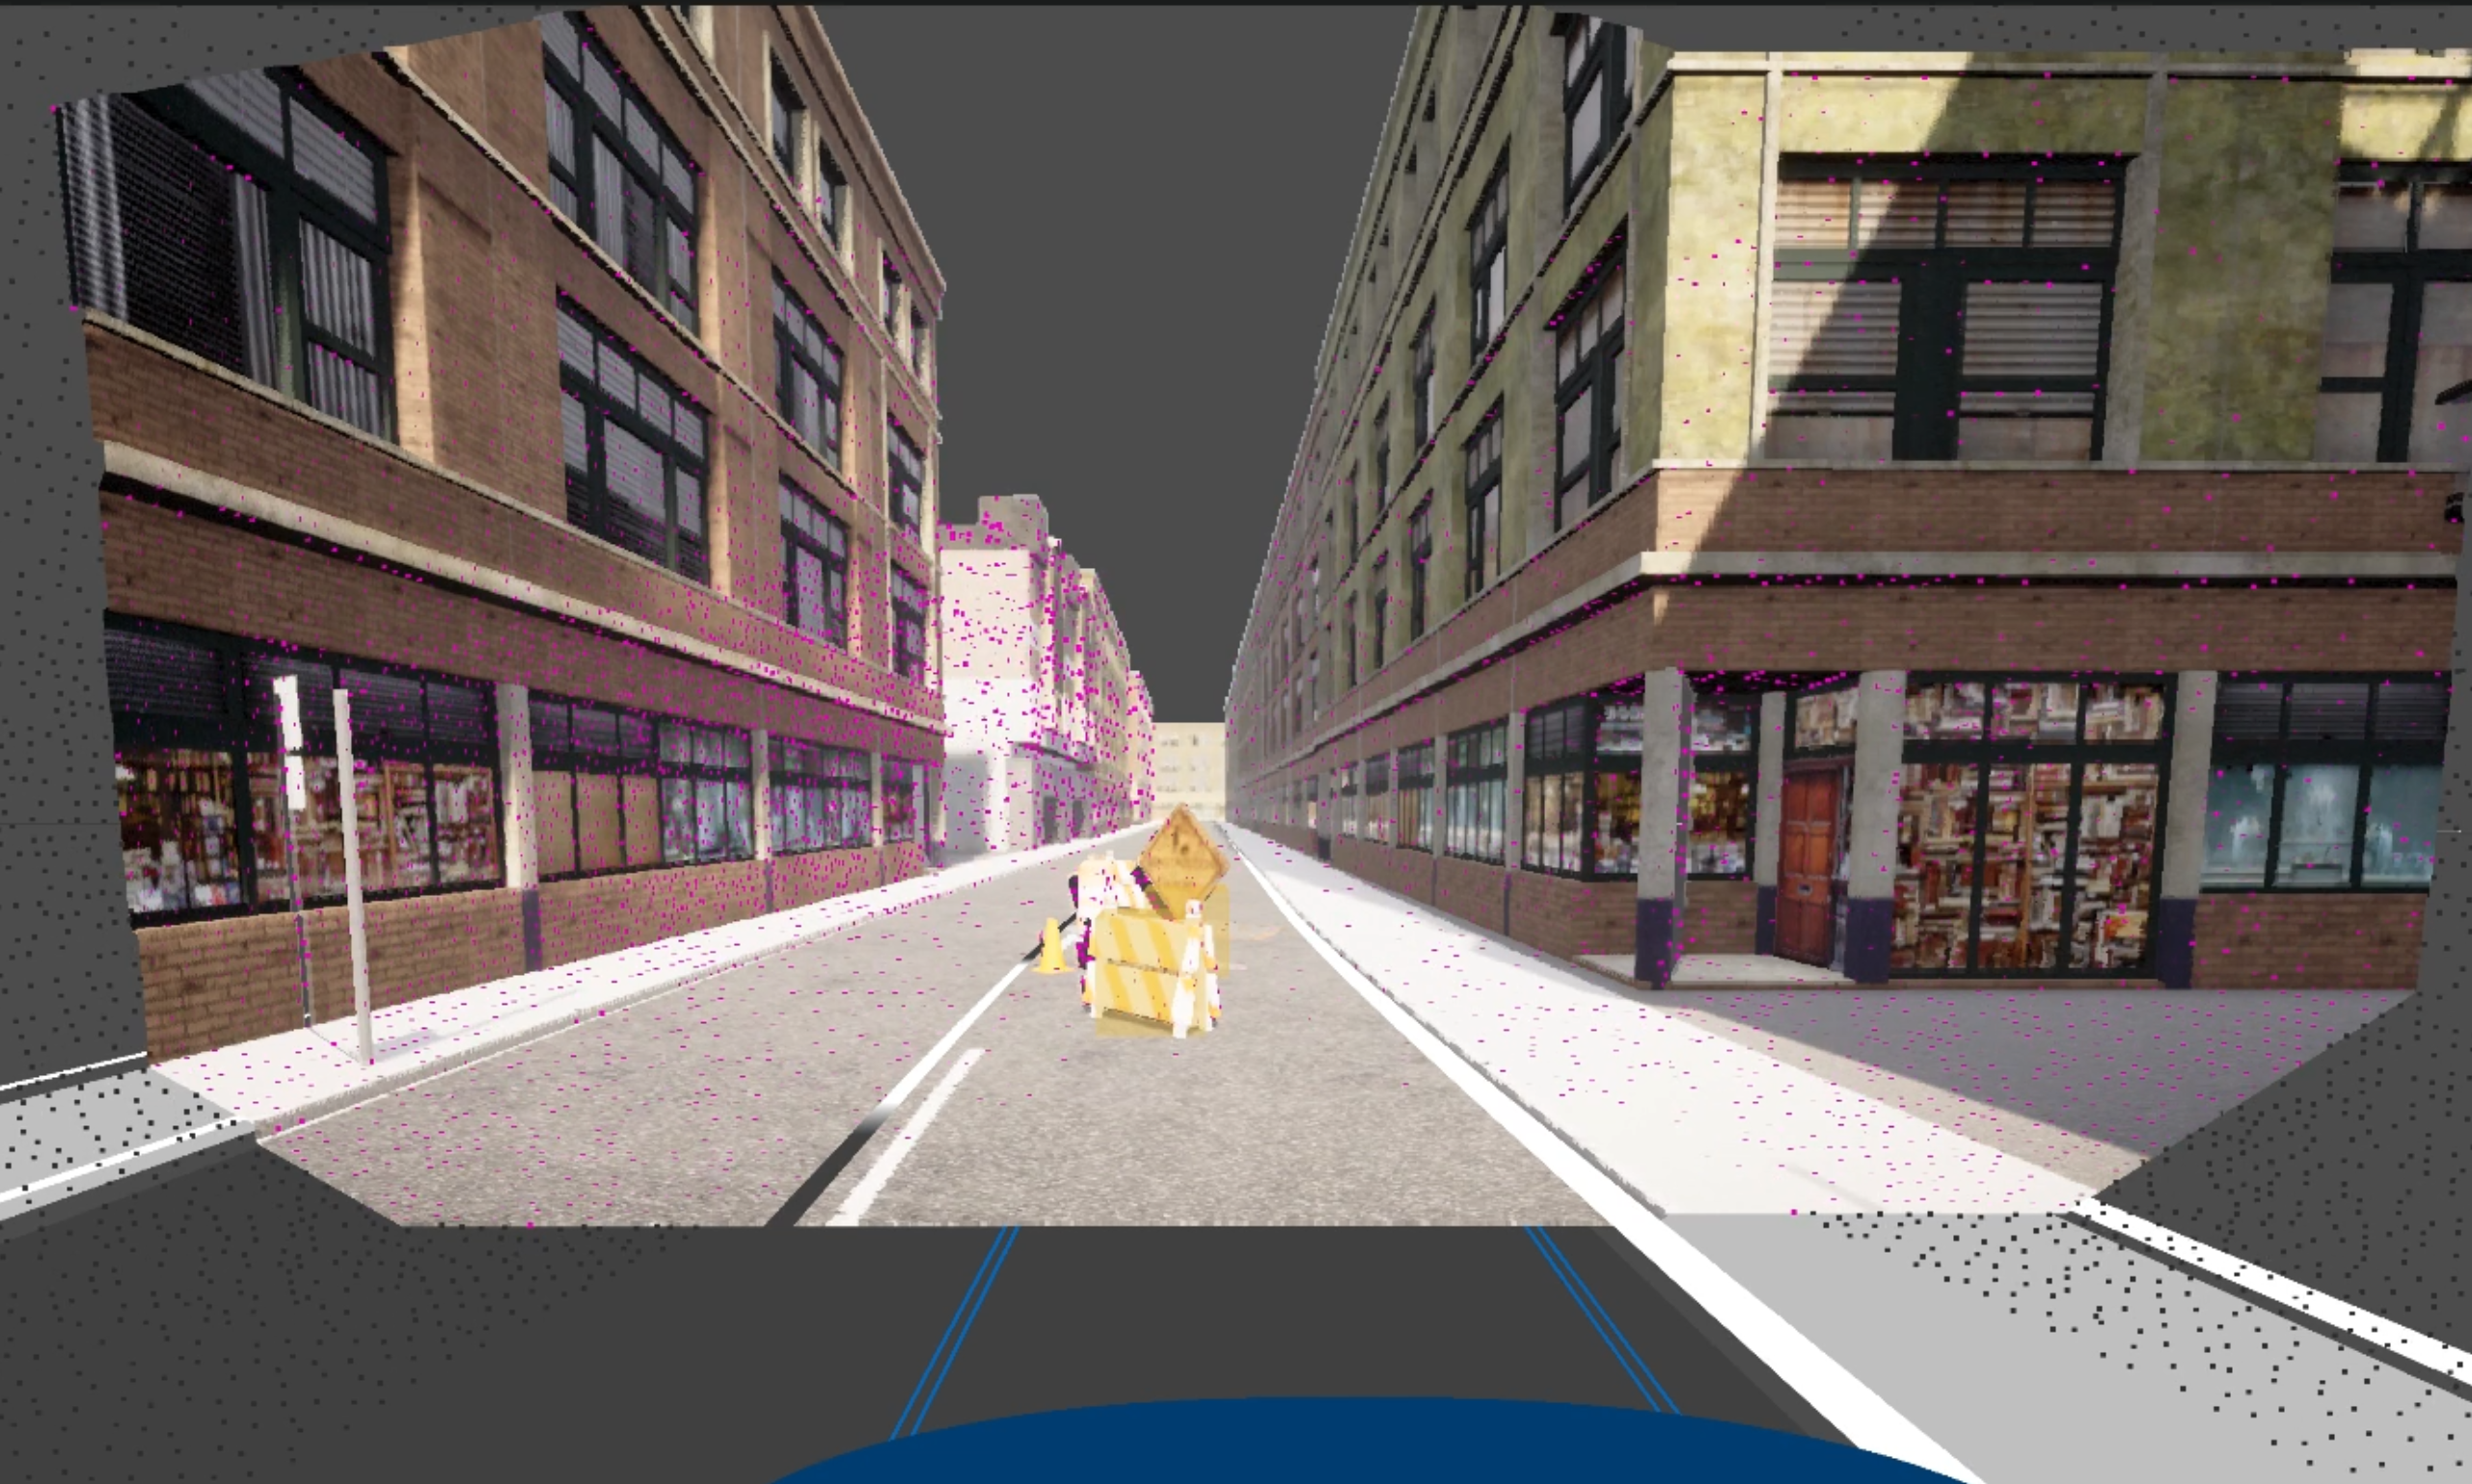
\includegraphics[width=\textwidth]{figures/scenario_cons.png}
        \caption{Construction site scenario}
        \label{fig:scenario_construction}
    \end{subfigure}
    \hfill
    \begin{subfigure}[b]{0.45\textwidth}
        \centering
        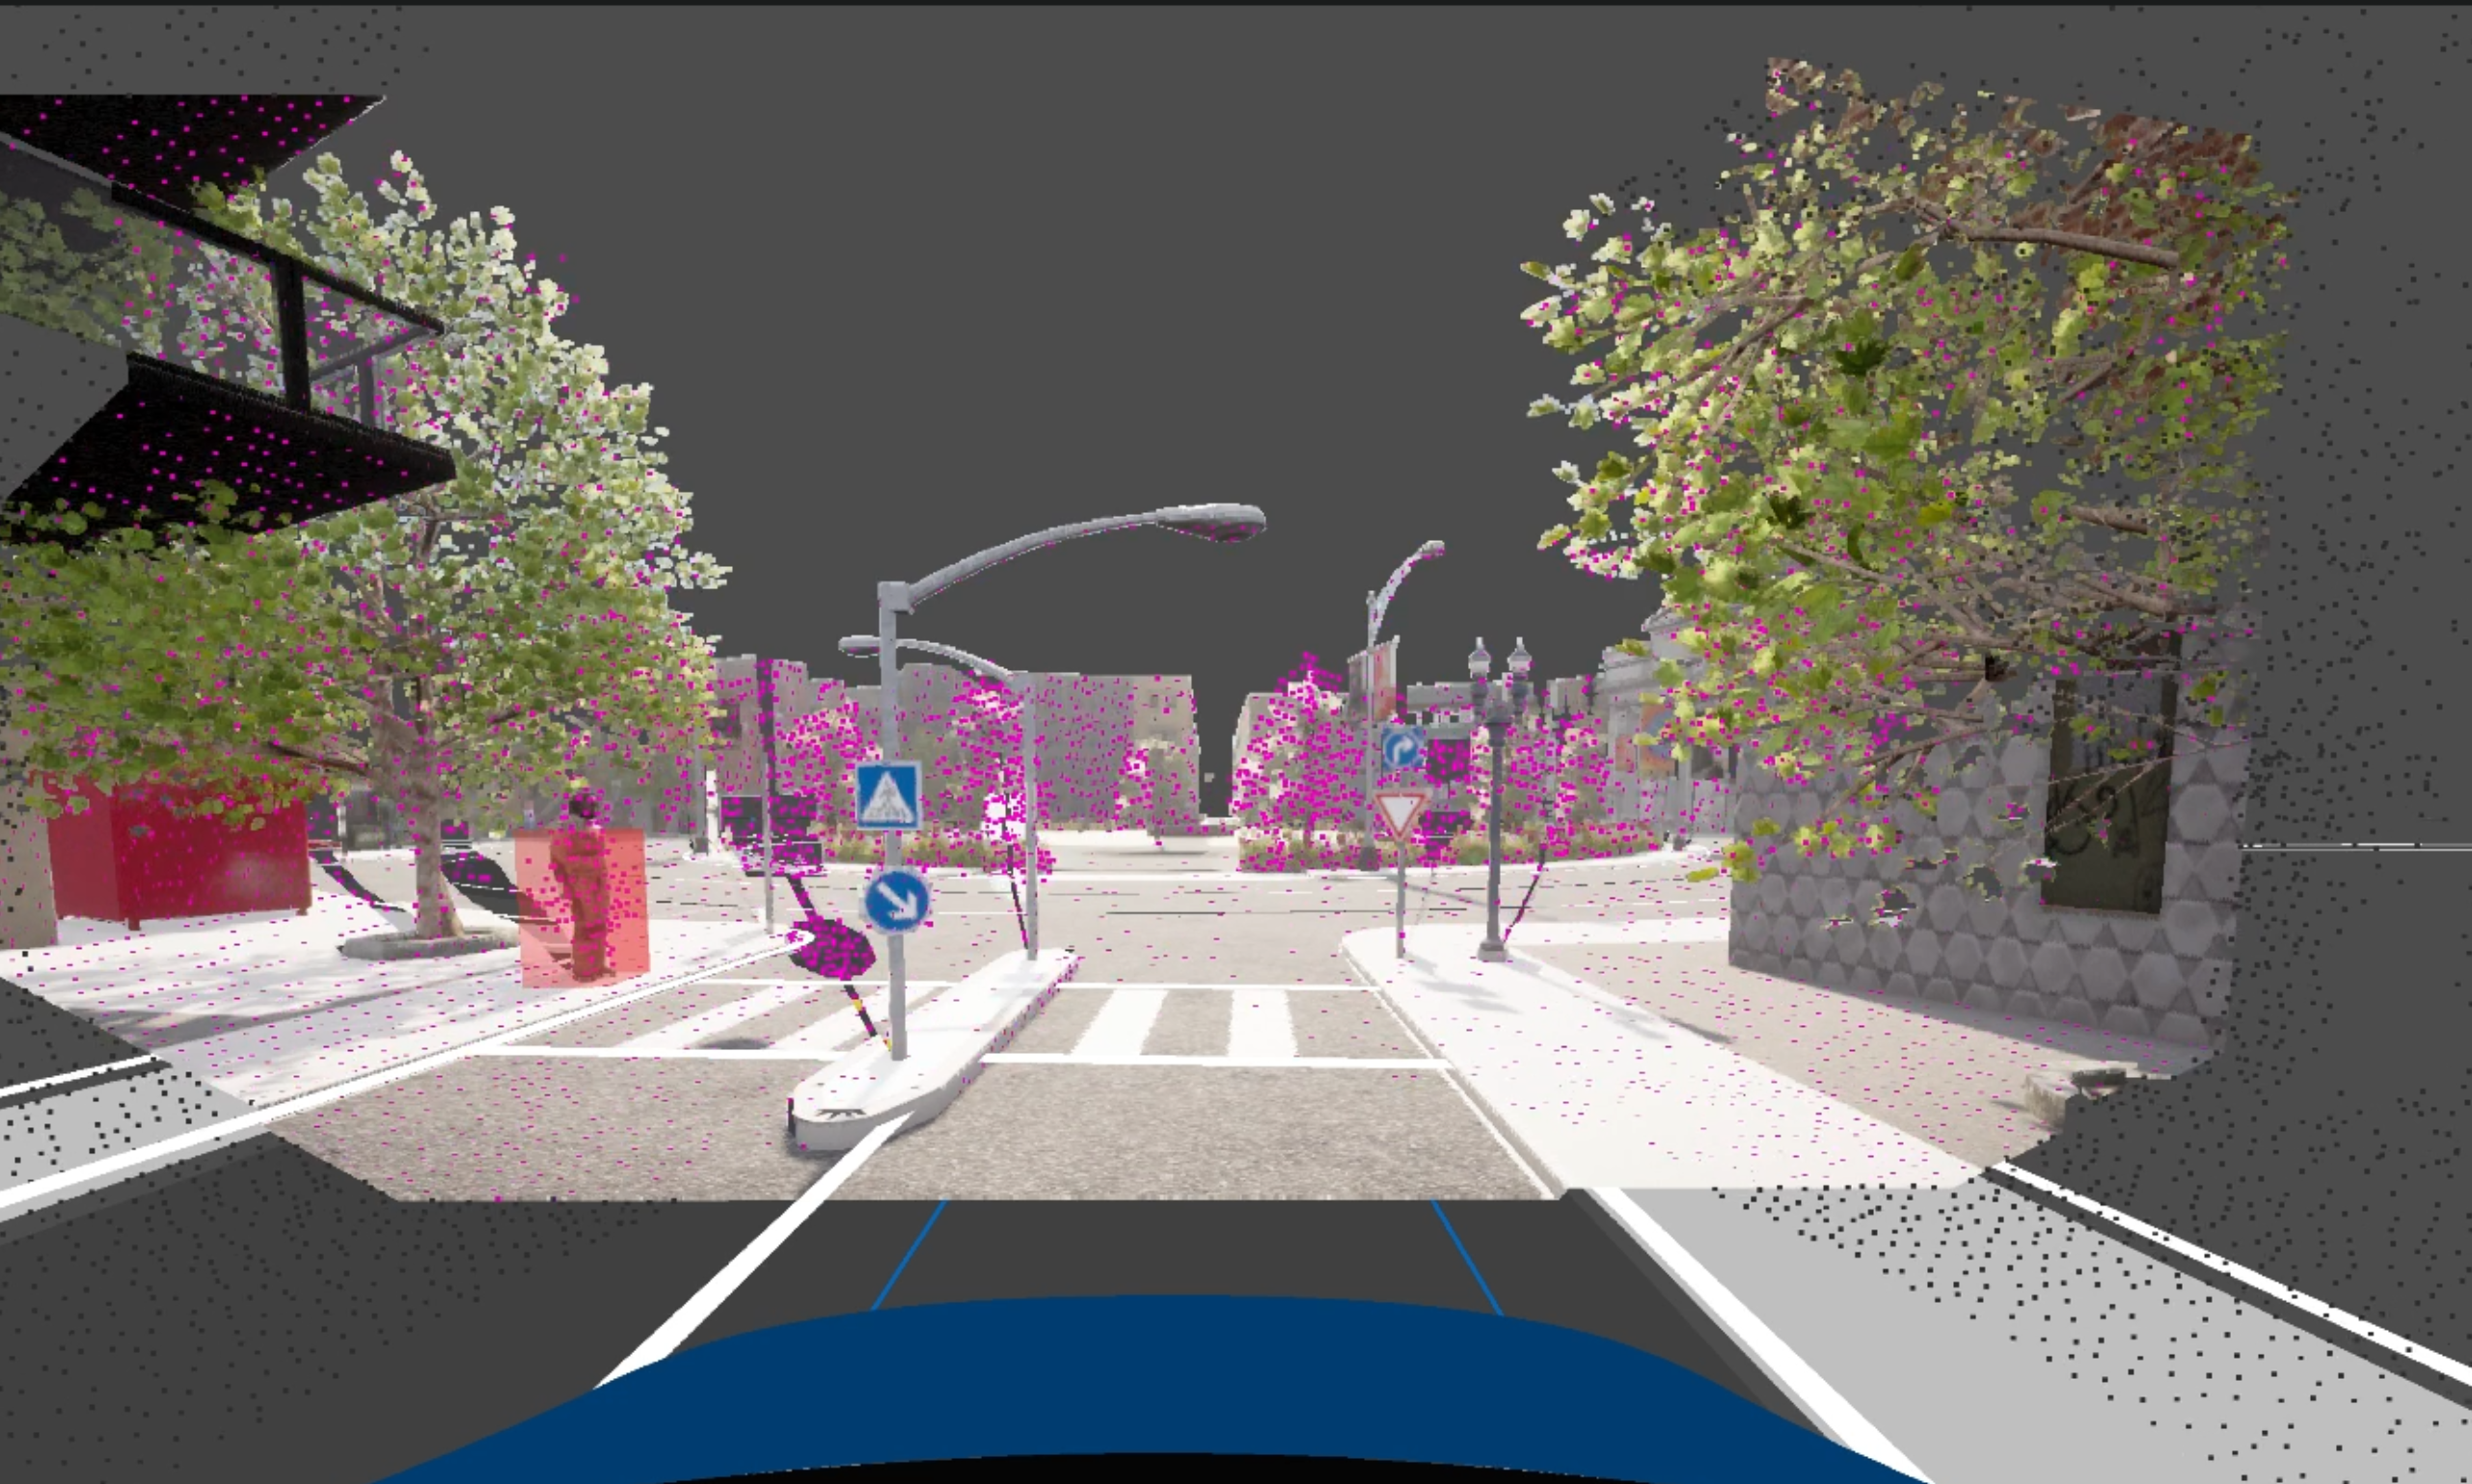
\includegraphics[width=\textwidth]{figures/scenario_cross.png}
        \caption{Pedestrians at a crosswalk scenario}
        \label{fig:scenario_crosswalk}
    \end{subfigure}
    \newline
    \begin{subfigure}[b]{0.45\textwidth}
        \centering
        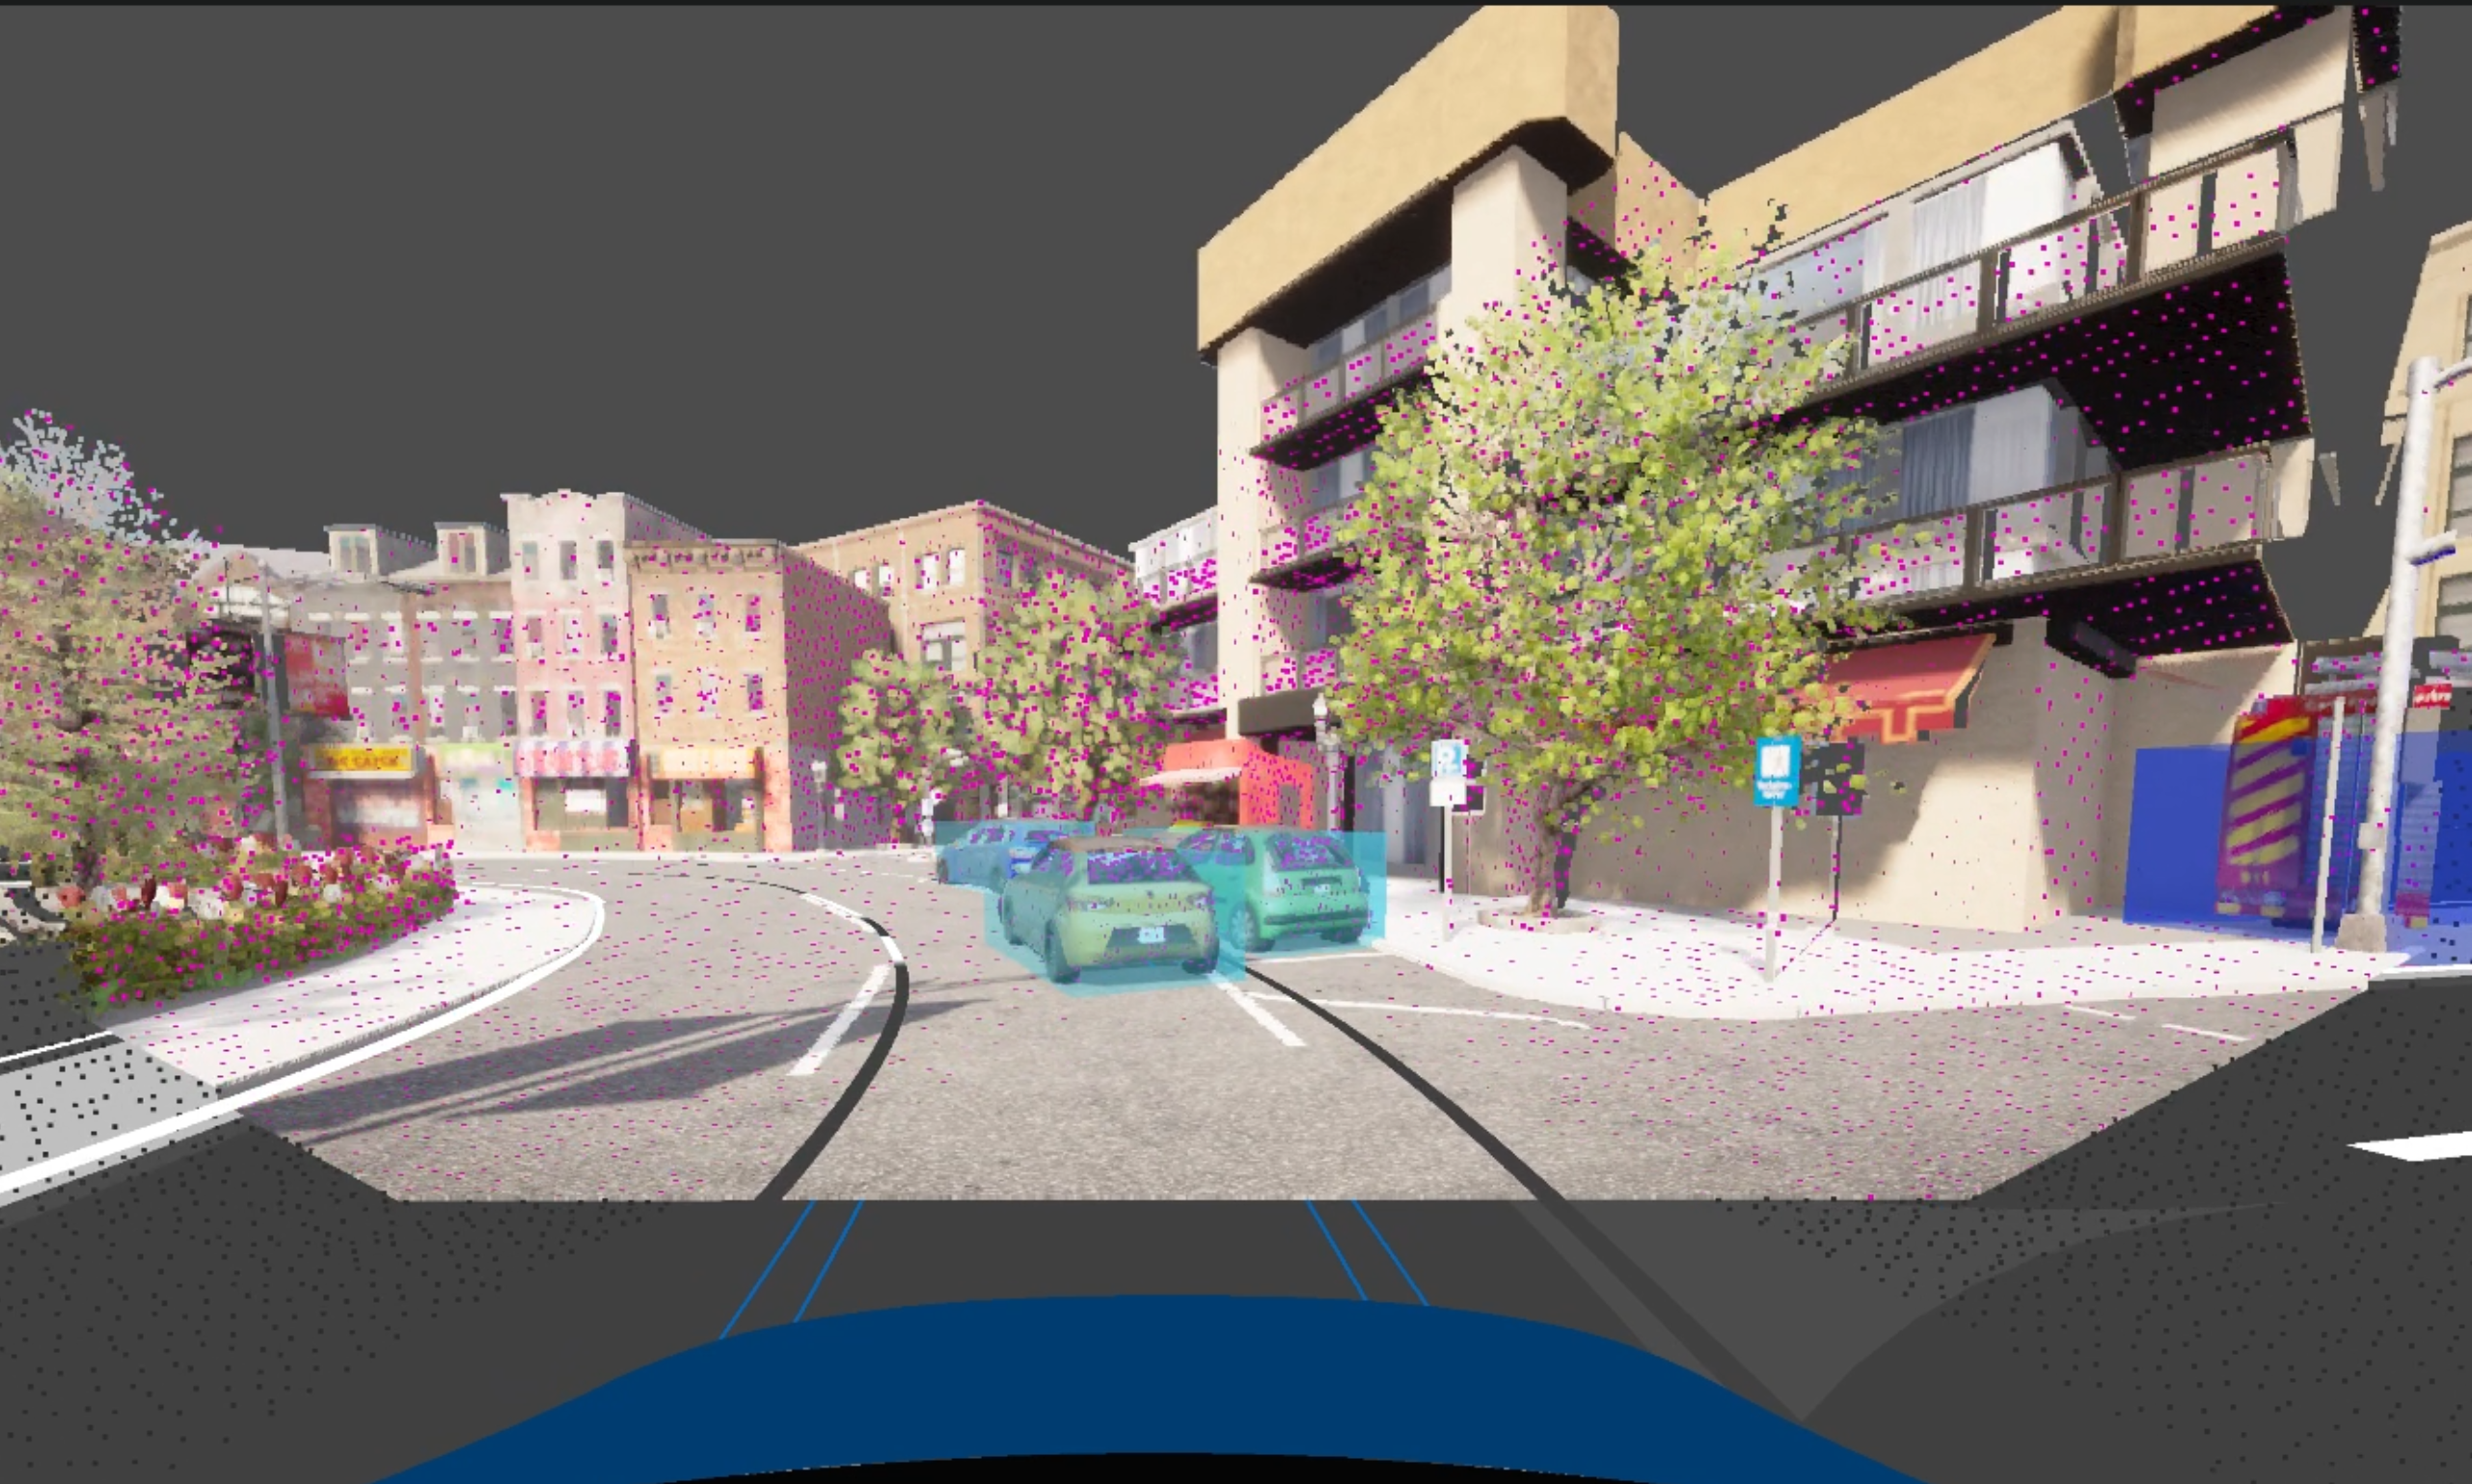
\includegraphics[width=\textwidth]{figures/scenario_srp.png}
        \caption{Second row parker scenario}
        \label{fig:scenario_srp}
    \end{subfigure}
    \hfill
    \begin{subfigure}[b]{0.45\textwidth}
        \centering
        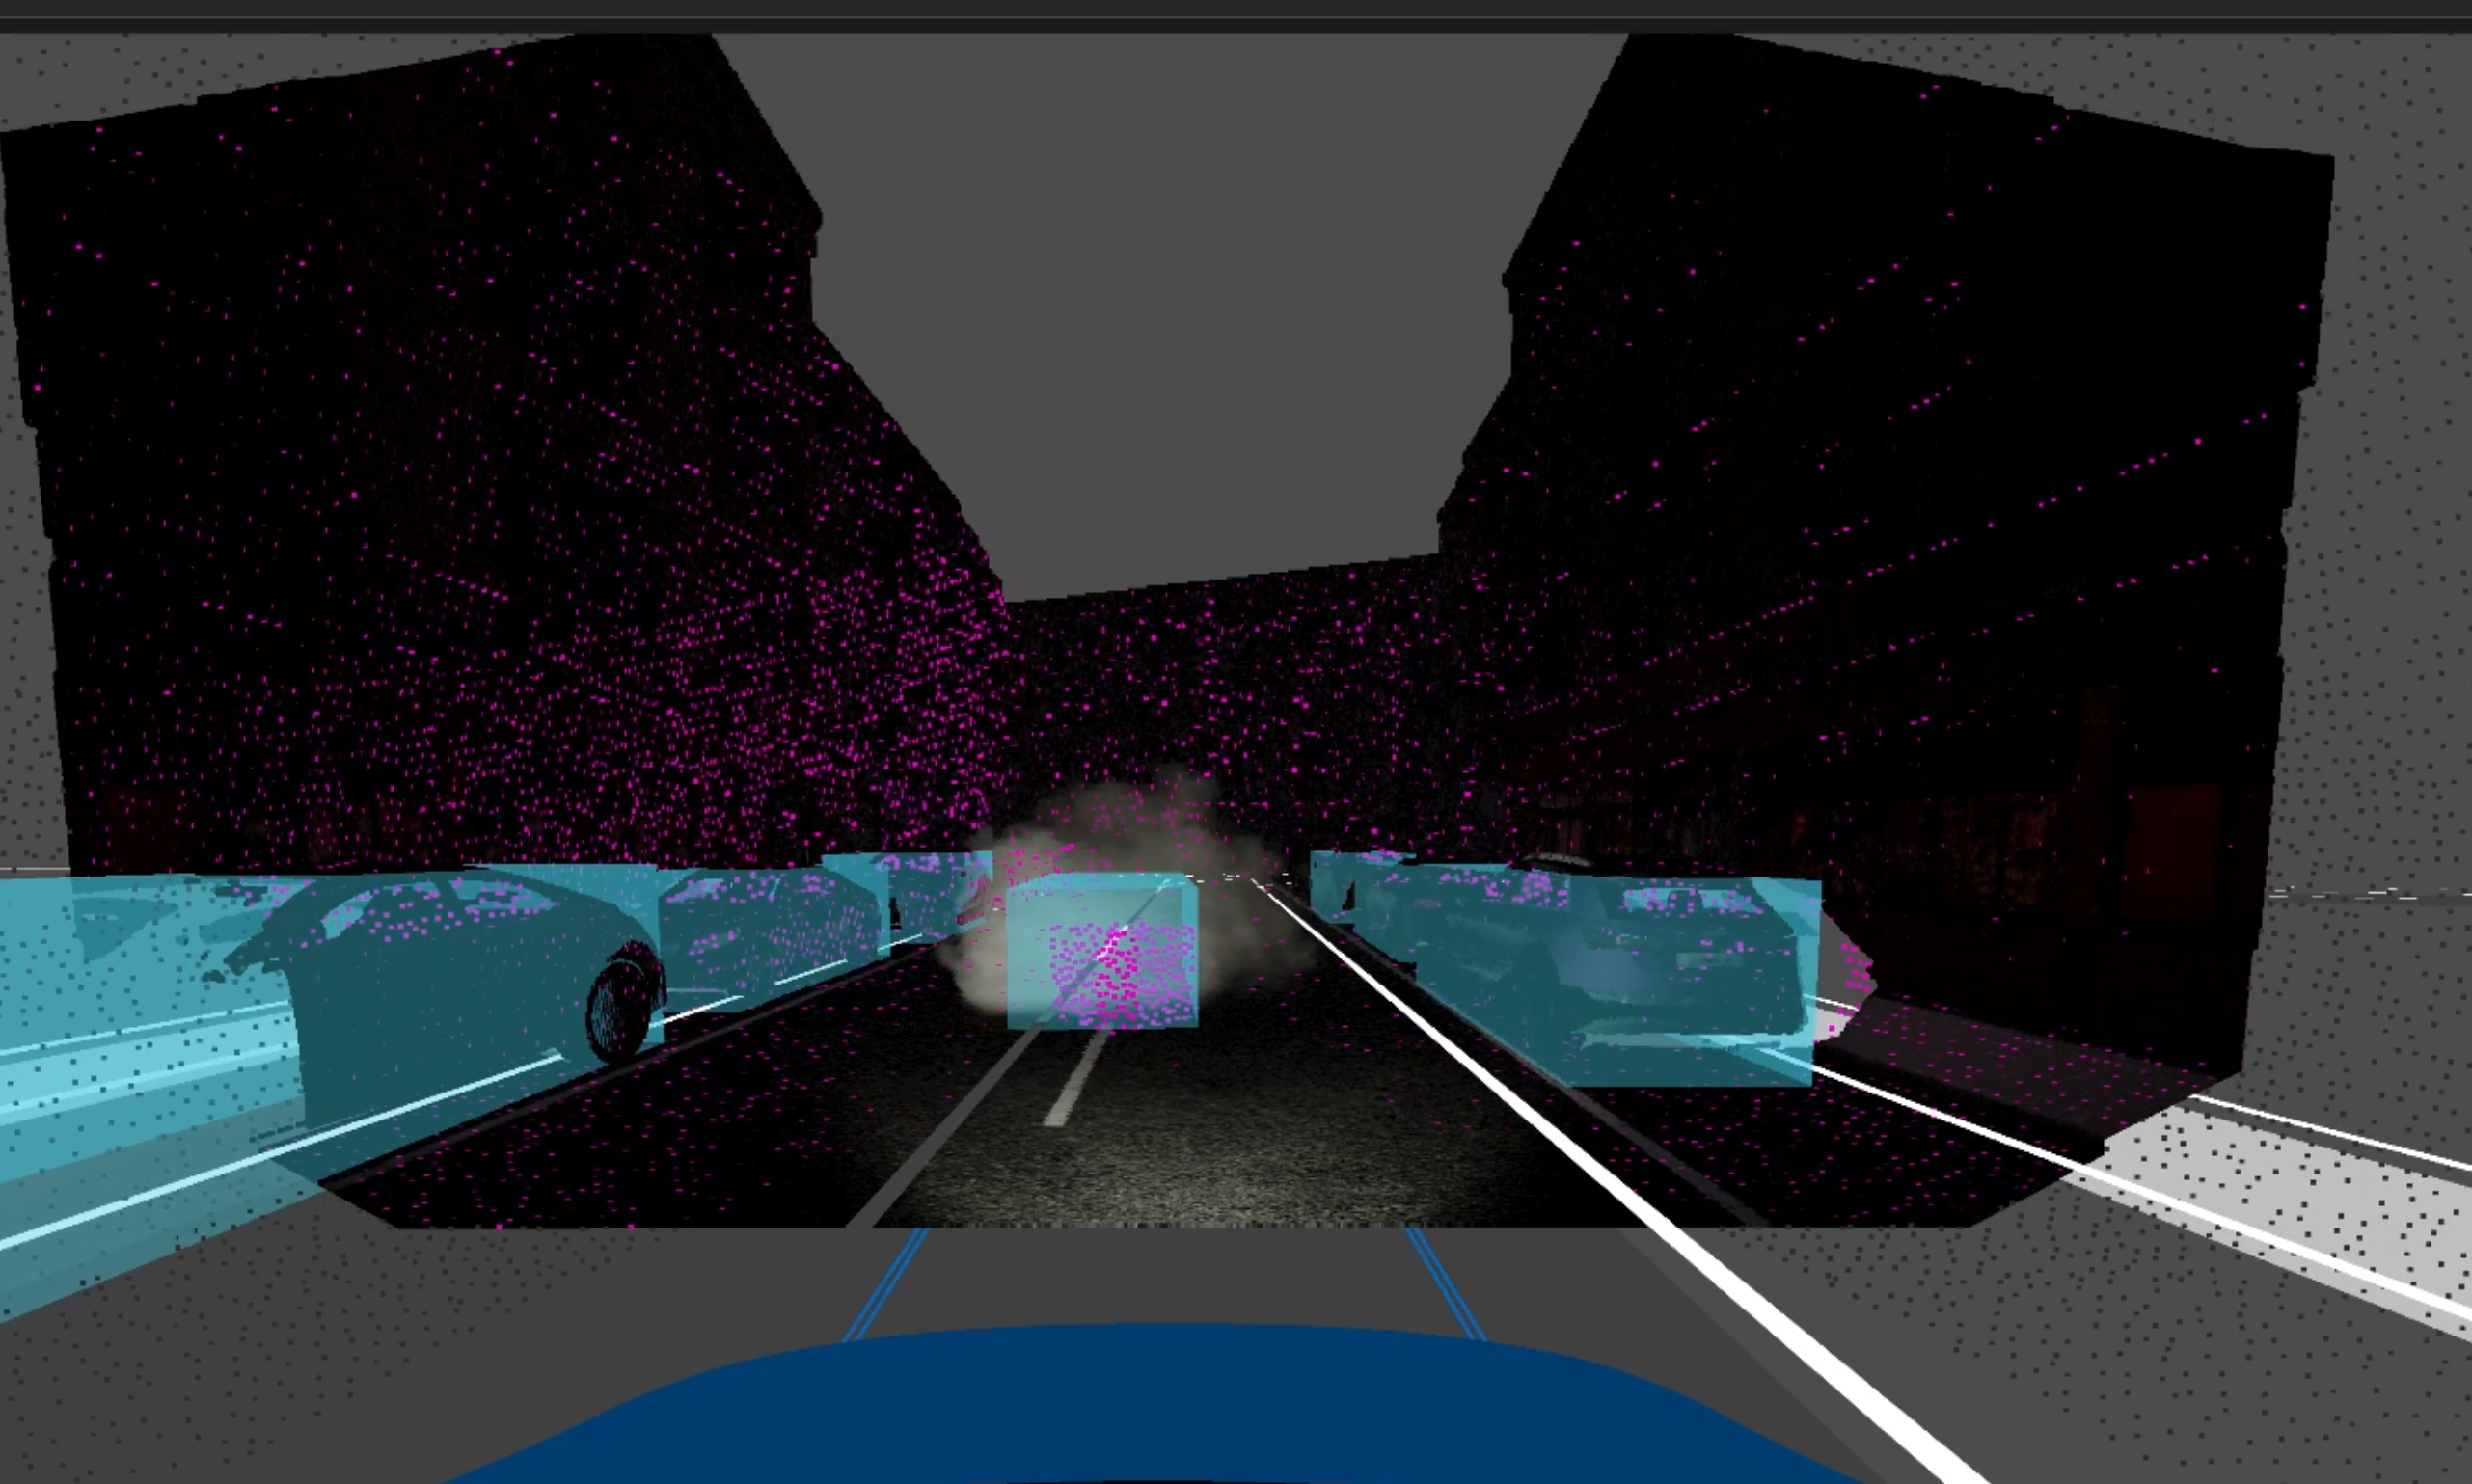
\includegraphics[width=\textwidth]{figures/scenario_smoke.png}
        \caption{Smoke from sewer scenario}
        \label{fig:scenario_smoke}
    \end{subfigure}
    \caption{Scenarios for object modification tasks}
    \label{fig:full}
\end{figure}


\subsection{Questionnaire}
The questionnaire for evaluating the visualization interfaces combines standardized assessment tools with custom questions specific to perception modification tasks. Developed by Tobias Kerbl, the questionnaire structure follows a comprehensive approach to gather both objective and subjective feedback from participants. For this thesis, we use a subset of the questions focusing on situational awareness, mental workload, and specific subjective evaluations to compare the interface variants.

The demographic section collects information about participants' backgrounds, including age, gender, driving experience, and familiarity with video games and technical systems. This data helps analyze whether certain user characteristics influence performance with different visualization approaches.

For assessing situational awareness, we employ the \ac{SAGAT}. The \ac{SAGAT} questions are customized for each scenario and cover all three levels of situation awareness: perception (Level 1), comprehension (Level 2), and projection (Level 3). This method, developed by Endsley \cite{endsley1988sagat}, allows for an objective measurement of participants' understanding of the current environment, their ability to integrate this information, and their capacity to predict future states. We slightly modified the original \ac{SAGAT} questions to better fit the perception modification tasks in our study. Our design consist of having one question for each level of situation awareness for each scenario.
\begin{table}[h!]
    \centering
    \begin{tabular}{|p{6cm}|p{7.8cm}|}
    \hline
    \textbf{SAGAT Level} & \textbf{Question} \\
    \hline
    Level 1 (Perception) & 4-5 statements per scenario. We expect the user to mark the correct ones. Example Statement: The vehicle trajectory was blocked by an undefined object. \\ \hline
    Level 2 (Comprehension) & Free-text question to question if the participants understand why the \ac{AV} stopped in the scenario \\ \hline
    Level 3 (Projection) & Multiple choice question that gives the possible outcomes after applying an operator modification on the scenario and measures the participants understanding on the vehicle behavior afterwards. \\ \hline
    \end{tabular}
    \caption{Questions to measure \ac{SA}}
    \label{table:scenariosunsolvable}
    \end{table}

Mental workload is evaluated using the \ac{NASA-TLX} \cite{hart1988development}, focusing on dimensions such as mental demand and frustration level. This tool, widely used in human factors research, provides insights into the cognitive demands placed on operators during teleoperation tasks.

After each interface variant, participants provide subjective feedback on usability and feature effectiveness. This includes evaluating specific visualization elements such as point cloud representation, bounding box visualization, traffic element rendering, and prediction visualization. These questions are designed to capture participants' perceptions of the interface's ability to support perception modification tasks.

The questionnaire concludes with comparative questions where participants rank the interface variants and provide qualitative feedback on their preferences and suggested improvements. This section aims to gather insights into which aspects of each interface were most effective and where improvements could be made.
\section{Study Preparation}

The preparation phase of our user study required careful attention to three key components to ensure consistent and reproducible results across all participants. This section details the systematic approach taken to create a controlled yet realistic testing environment.

First, we developed a custom simulation environment based on Munich's Gärtnerplatz square, moving away from generic or US-centric scenarios typical in autonomous driving research. The map creation process, detailed in Section \ref{section:mapcreationforcarla}, involved translating real-world geographical data into a format suitable for the CARLA simulator while maintaining the location's distinctive features.

Following the environment creation, we implemented a structured scenario recording workflow that combines CARLA simulation with Autoware's autonomous driving stack. This process, which presented several technical challenges in maintaining data quality while managing computational constraints, ensures that each test scenario is reproducible and consistent across different interface evaluations.

Finally, we developed a standardized video creation pipeline to ensure consistent scenario playback across the three interface variants. This step was crucial in ensuring that participants could evaluate all three interface variants - the Separate View, Integrated View, and Integrated View with Ground Truth - under identical conditions.

The following subsections detail each of these preparation steps, describing the technical implementation, challenges encountered, and solutions developed to create a robust experimental framework.


\subsection{Map creation for CARLA}\label{section:mapcreationforcarla}
To ensure the ecological validity of our user study and provide a realistic simulation environment, we developed a custom map for CARLA based on the Gärtnerplatz square in Munich, Germany. This section describes the map creation process, which involved replicating the real-world location as closely as possible while adapting it to the capabilities of the CARLA simulator.
\subsubsection*{Pipeline Overview}
\begin{figure}
    \centering
    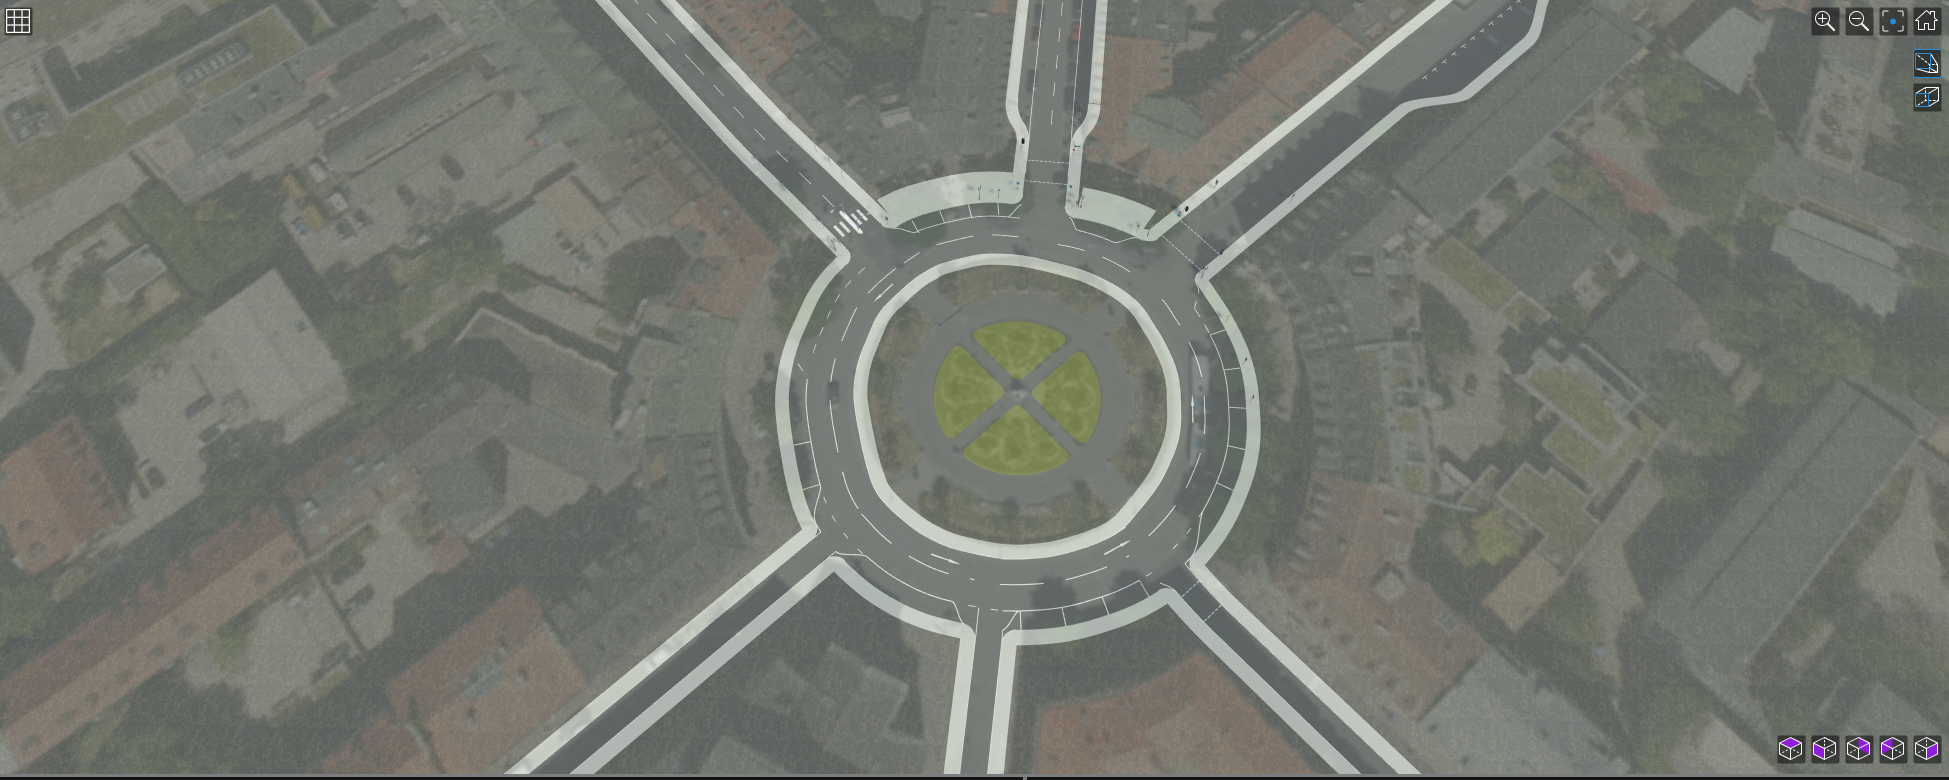
\includegraphics[width=\textwidth]{figures/roadrunner.png}
    \caption{Road network design of Gärtnerplatz in MathWorks RoadRunner}
    \label{fig:roadrunner}
\end{figure}
The map creation process followed a structured pipeline:
\begin{enumerate}
    \item Road Network Creation: Using MathWorks RoadRunner, we designed the road network based on satellite data obtained from the Geoportal Bayern \cite{geoportal_bayern}. The road network included all major features of Gärtnerplatz, such as the six-way roundabout, one-way roads, two-way roads with traffic islands, and traffic lights at intersections. Regulatory elements like crosswalks, traffic signs, and lane markings were added to align with real-world traffic rules. The results can be seen in Result can be seen in \ref{fig:roadrunner}.
    \item Export to OpenDRIVE: The road network and regulatory elements were exported in OpenDRIVE format using RoadRunner's export tools \cite{mathworks_roadrunner}.
    \item Import into Unreal Engine: The OpenDRIVE file and associated assets were imported into Unreal Engine using CARLA's RoadRunner import plugin \cite{carla_map_import}. This step included setting up the road geometry, lane configurations, and traffic rules within CARLA's simulation environment.
    \item Environment Art: Additional environment details, such as buildings, vegetation, and textures, were created in Unreal Engine using CARLA's default asset set. The visual elements were designed to replicate the appearance of Gärtnerplatz as closely as possible.
\end{enumerate}

\begin{figure}[h]
    \centering
    \begin{subfigure}{\textwidth}
        \centering
        \includegraphics[width=\textwidth, trim=0 200pt 0 200pt, clip]{figures/sim_top.png}
        \caption{Top view of the simulation environment}
        \label{fig:sim_top}
    \end{subfigure}
    \begin{subfigure}{\textwidth}
        \centering
        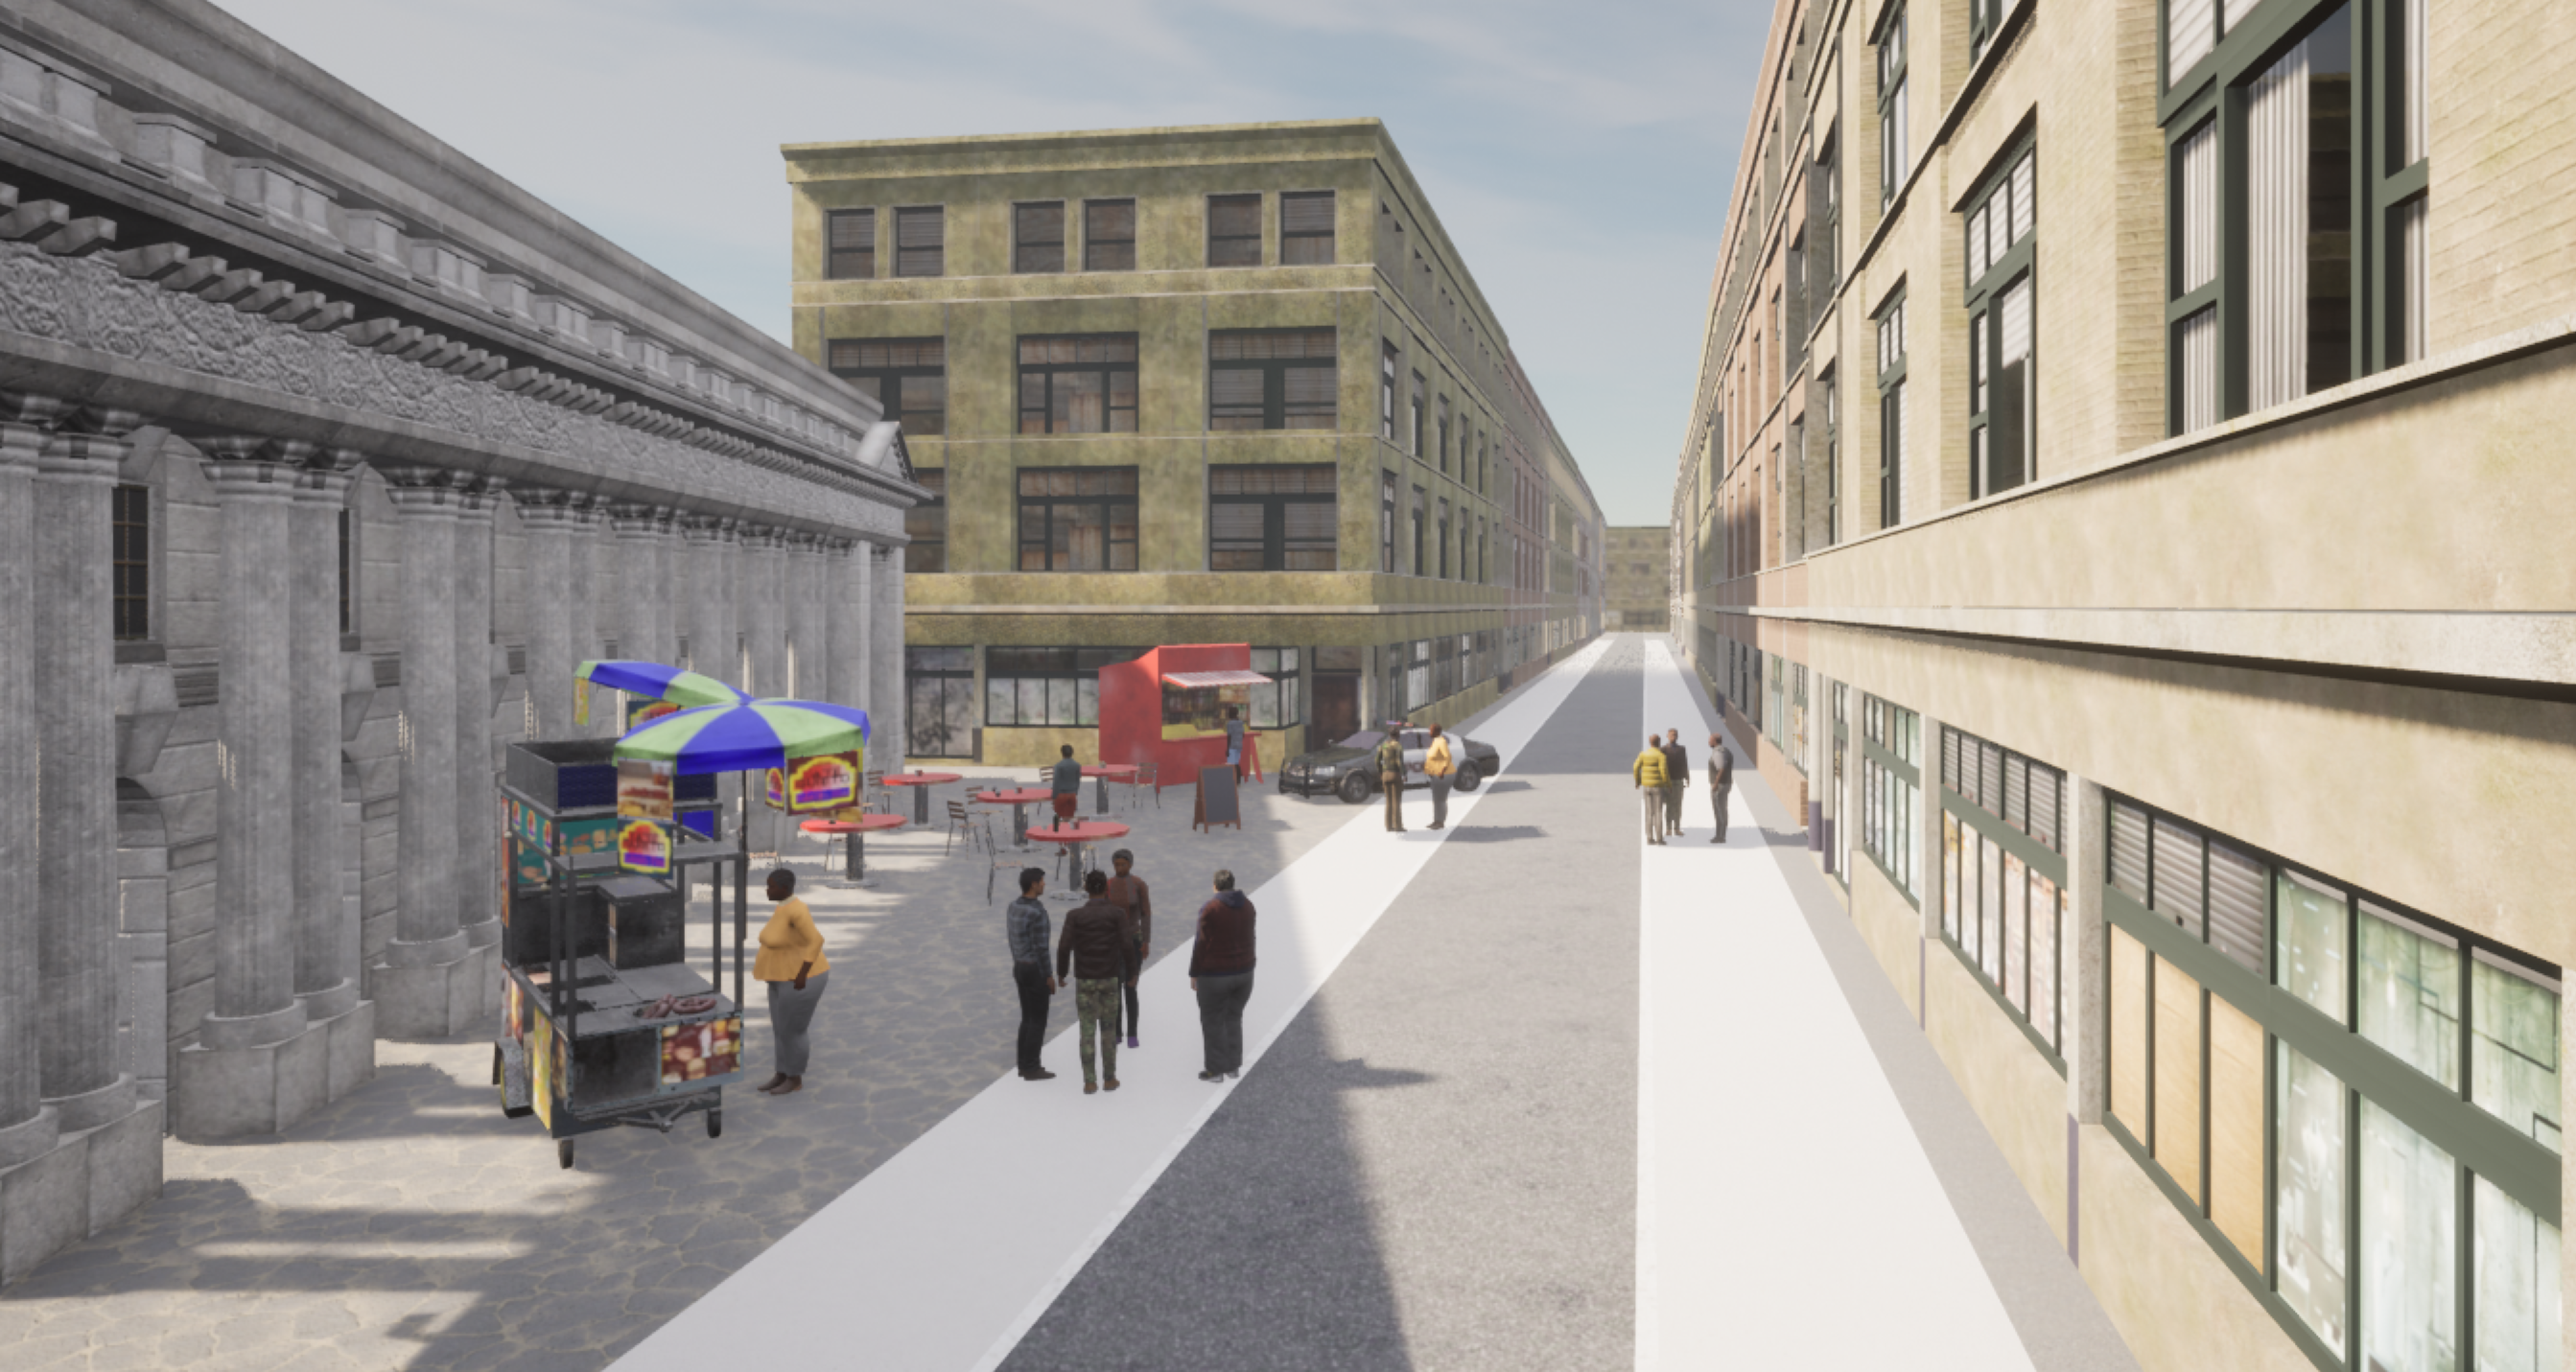
\includegraphics[width=\textwidth, trim=0 200pt 0 200pt, clip]{figures/sim_crowd.png}
        \caption{Environment is detailed to provide a dynamic city look}
        \label{fig:sim_crowd}
    \end{subfigure}
    \begin{subfigure}{\textwidth}
        \centering
        \includegraphics[width=\textwidth, trim=0 200pt 0 200pt, clip]{figures/sim_signs.png}
        \caption{Local traffic signs are used in their real-world locations}
        \label{fig:sim_signs}
    \end{subfigure}
    \caption{Simulation environment based on Gärtnerplatz square}
    \label{fig:simulation}
\end{figure}
\FloatBarrier
\subsubsection*{Real-World Location Selection}
The Gärtnerplatz square was selected due to its unique traffic layout and diverse road types. Table~\ref{table:gaertnerplatz_features} summarizes the key features of this location.

\begin{table}[h!]
\centering
\begin{tabular}{@{}p{4cm}p{10cm}@{}}
\toprule
\textbf{Feature} & \textbf{Description} \\
\midrule
Six-way roundabout & A central roundabout with six connecting roads, creating a complex traffic layout. \\
\midrule
One-way roads & Roads leading in different directions, adding diversity to traffic flow patterns. \\
\midrule
Two-way roads & Includes traffic islands and signalized intersections for managing bidirectional traffic. \\
\midrule
Central square & Surrounded by buildings, creating a visually complex and busy scene. \\
\bottomrule
\end{tabular}
\caption{Key Features of Gärtnerplatz Square}
\label{table:gaertnerplatz_features}
\end{table}

These features highlight why Gärtnerplatz was chosen as the location for our study. Its diverse traffic layouts and visually complex environment provide an excellent basis for evaluating teleoperation interfaces under realistic conditions.

Satellite imagery from Geoportal Bayern \cite{geoportal_bayern} served as the basis for road layout design. Google Maps' Street View feature was used to identify traffic signs, building types, and vegetation patterns. These references ensured that the map accurately reflected real-world conditions while remaining computationally efficient for simulation.

\subsubsection*{Challenges and Adaptations}
While we aimed to replicate Gärtnerplatz accurately, certain adaptations were necessary due to computational constraints. Table~\ref{table:challenges_adaptations} summarizes these challenges and the corresponding adaptations.

\begin{table}[h!]
\centering
\begin{tabular}{@{}p{4cm}p{10cm}@{}}
\toprule
\textbf{Challenge} & \textbf{Adaptation} \\
\midrule
Rendering Overhead & Simplified building models and vegetation to reduce computational load. \\
\midrule
Road Geometry & Adjustments to road curvature and lane widths to meet CARLA's simulation requirements. \\
\midrule
Asset Compatibility & Replacement of real-world objects with CARLA's default textures and assets. \\
\bottomrule
\end{tabular}
\caption{Challenges and Adaptations for Gärtnerplatz Map in CARLA}
\label{table:challenges_adaptations}
\end{table}

These adaptations ensured that the map remained computationally efficient while preserving key features relevant to our user study scenarios. By creating a map tailored to our study's requirements, we provided participants with a realistic yet controlled simulation environment for evaluating teleoperation interfaces.
\subsection{Scenario Recording}
The scenario recording process involves multiple components working together to create reproducible test cases for our user study. We developed a systematic workflow that ensures consistent and high-quality recordings of each scenario while managing computational constraints.

The process begins with Python scripts that set up the simulation environment. These scripts configure the scene by loading the appropriate map, placing vehicles in predetermined positions, and spawning dynamic props relevant to each scenario. Once the CARLA simulation is running, we initiate the CARLA-Autoware Bridge, which configures the sensor suite on our test vehicle and establishes the necessary ROS message pipeline for Autoware.

Autoware runs in "ghost mode" during recording, meaning that while all perception, planning, and localization modules function normally, we override the control commands. Instead of using Autoware's autonomous control, we manually control the vehicle through our custom UI to precisely recreate each scenario.

The scenarios are recorded using rosbag, ROS's built-in data logging system that captures and stores message data from specified topics. Rosbag files contain timestamped sensor data, perception outputs, and vehicle states, allowing for exact replay of scenarios during the user study.

However, the recording process presented significant computational challenges. The overhead of recording rosbag files while running the full simulation stack caused performance degradation that prevented real-time operation. To address this, we implemented a workaround using CARLA's time management features:

\textbf{During recording:} We decoupled the simulation time from real-time constraints, allowing approximately one second of computation time per frame

\textbf{During replay:} We utilize simulation time flags to achieve real-time playback

This approach ensures high-quality recordings while preserving all necessary data for scenario reproduction. It's important to note that this performance limitation only affects the recording process - the actual teleoperation system maintains real-time performance during normal operation.

\subsection{Video Creation}
The final step in preparing for the user study is creating videos for each scenario. These videos serve as the primary stimuli for participants, providing a consistent and controlled environment for evaluating the teleoperation interfaces. The video creation process involves several key components.

After obtaining the rosbag recordings from the scenario recording step, we implemented a systematic approach to create standardized video content. We played back each recorded scenario through three distinct interface configurations: the Separate View, the Integrated View, and the Integrated View with Ground Truth.

Using OBS Studio \cite{obs2024}, we captured high-quality screen recordings of each interface's display during scenario playback. To ensure consistency and optimal viewing experience, we maintained a standardized recording format across all scenarios while ensuring clear visibility of all interface elements. The recordings preserved the original resolution and frame rate to maintain visual fidelity, and we carefully eliminated any external distractions or unnecessary elements from the recordings.

The resulting video set provides participants with identical scenario presentations through all three interface variants, enabling direct comparisons during the user study. Each video underwent careful review to verify that all essential interface elements and scenario details were properly captured and clearly visible. These recordings form the foundation for our user study, allowing participants to experience all interfaces under identical conditions while maintaining experimental control. This approach ensures that any observed differences in participant responses can be attributed to the interface design rather than variations in scenario execution.